\section{Results}\label{paperB:sec:results}

In this section, we begin by providing the details about the collected dataset, which we have named the Grocery Store dataset. Furthermore, we illustrate the utility of the additional information in the Grocery Store dataset to classify grocery items in the experiments. We compare SplitAE, VCCA, and VCCA-private with different combinations of views against two standard image classifiers. Additionally, we experiment with a vanilla autoencoder (denoted as AE) and a VAE that post-processes the natural image features to train a linear classifier cheaper and compare the performance against the multi-view models. We measure the classification performance on the test set for every model and also compare the classification accuracies when the number of words in the text description varies for the models concerned (see subsection Classification Results in Results).
%(Section \ref{sec:classification_results}).
To gain insights on how the additional views affect the learned representations, we visualize the latent spaces of VCCA and VCCA-private with PCA and discuss how different views changes the structure of the latent space (see subsection Investigation of the Learned Representations in Results).
%(Section \ref{sec:investigation_of_the_learned_representations}).
Finally, we show how iconic images can be used for enhancing the interpretability of the classification (see subsection Decoding Iconic Images from Unseen Natural Images in Results),
%(Section \ref{sec:decoding_iconic_images}), 
which was also illustrated by Klasson \etal~\citeB{B:klasson2019hierarchical}.


\subsection{The Grocery Store Dataset}
\label{paperB:sec:grocery_store_dataset}

%%% Figure 3

\begin{figure}[t]
    \centering
    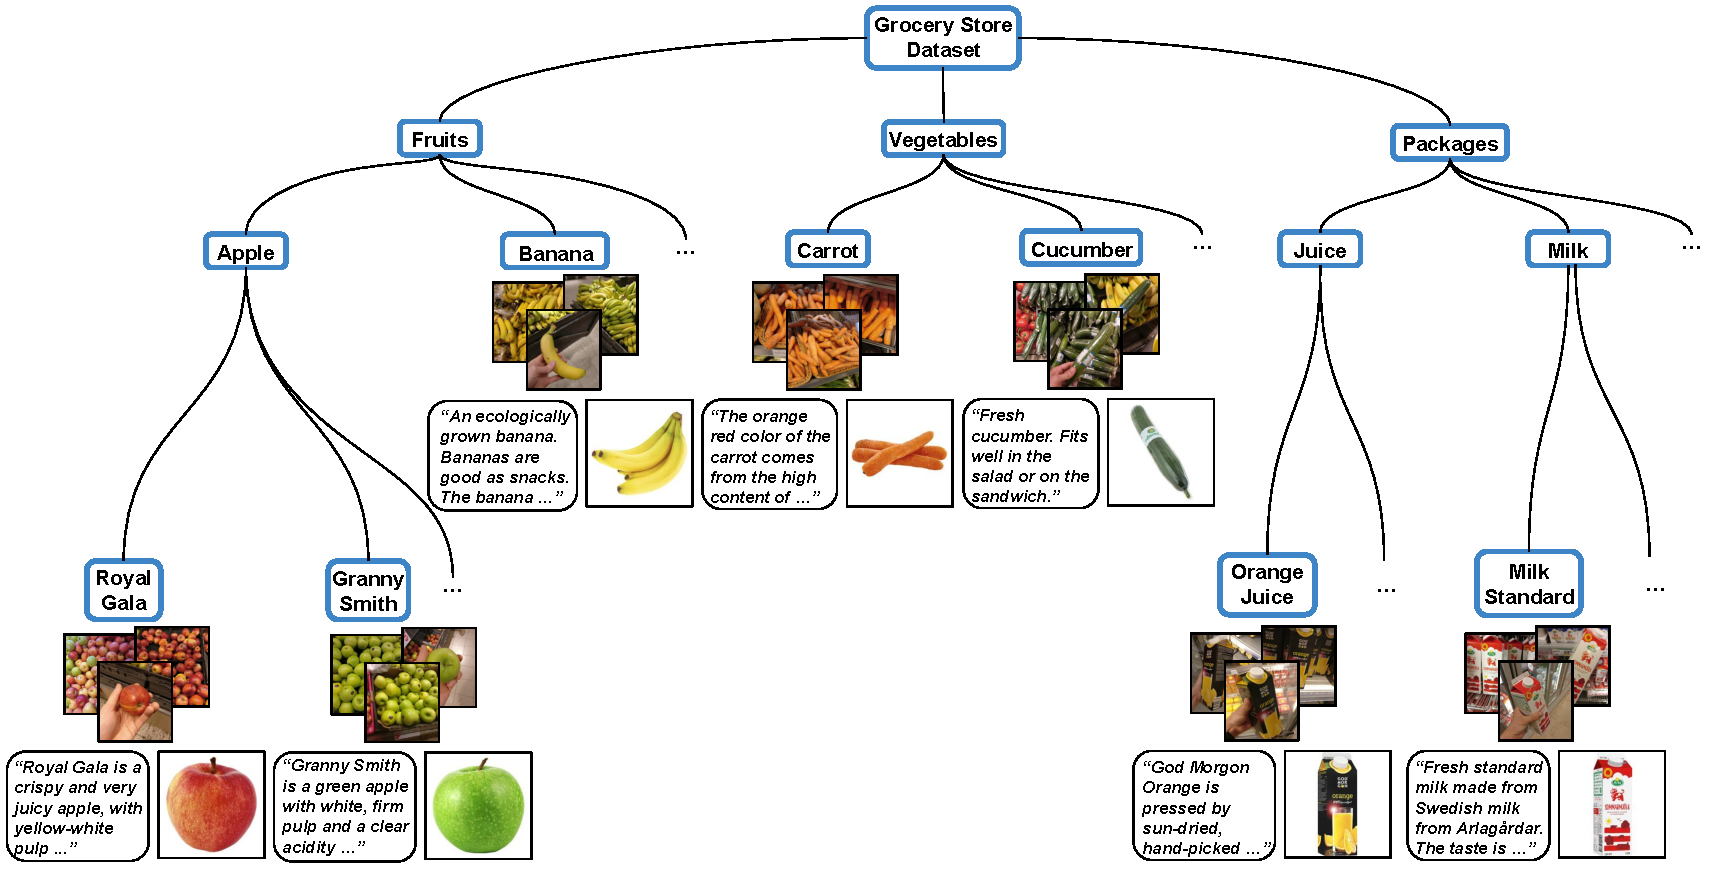
\includegraphics[width=\textwidth]{PaperB/figures_and_tables/dataset_figures/dataset_figure_new.pdf} %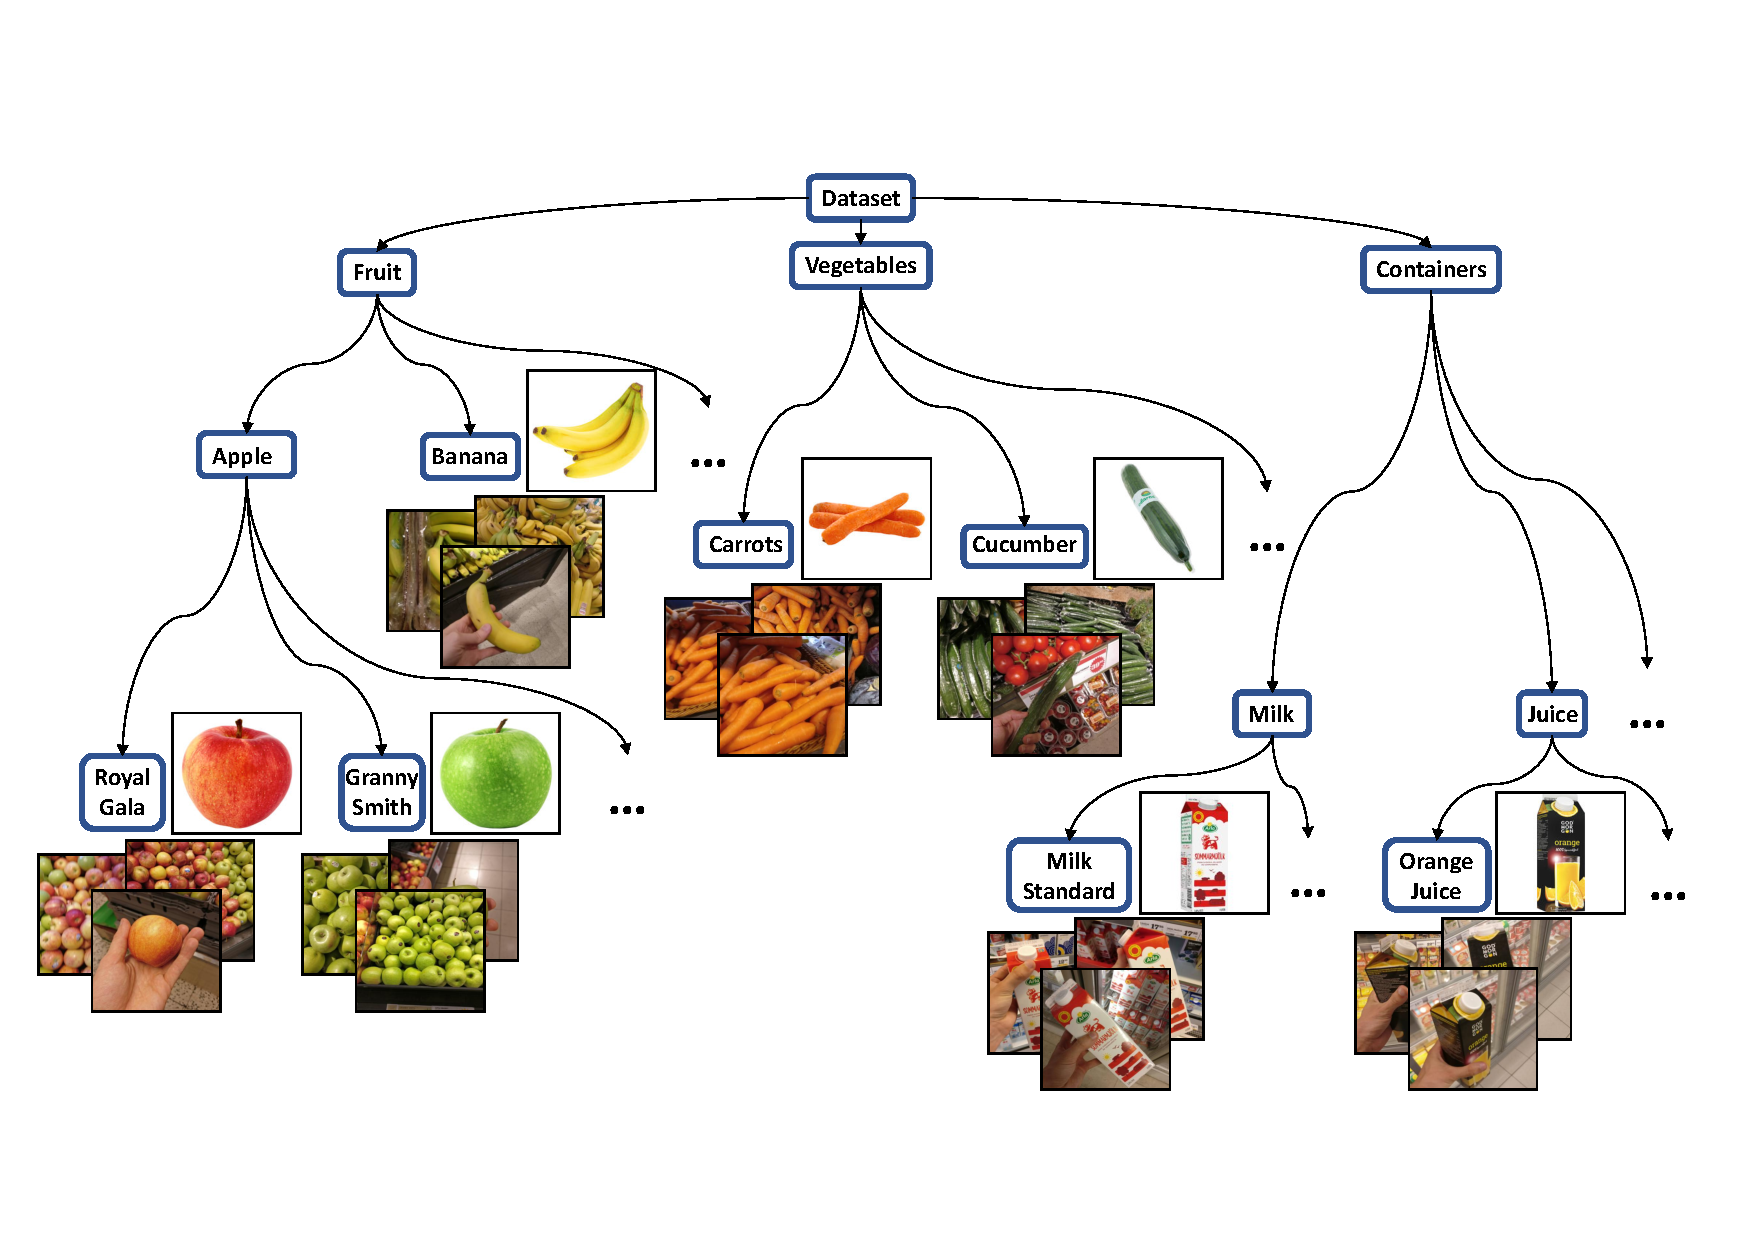
\includegraphics[width=0.95\textwidth]{dataset_figures/intro.pdf}
    \vspace{-2mm}
    \caption{Illustration of the hierarchical class structure of the dataset. First, the classes are divided by their grocery item type, i.e., \textit{Fruits}, \textit{Vegetables}, and \textit{Packages}, followed by a separating the items into coarse-grained classes, e.g., \textit{Apple}, \textit{Carrot}, and \textit{Milk}, and then into fine-grained classes. There are 81 fine-grained classes in total and 46 coarse-grained classes. The figure also shows the iconic image and text description of the items next to the class label.
   }
    \label{fig:examples} 
\end{figure}

In Klasson \etal~\citeB{B:klasson2019hierarchical}, we collected images from fruit, vegetable, and refrigerated sections with dairy and juice products in 20 different grocery stores.
The dataset consists of 5421 images from 81 different classes. For each class, we have downloaded an iconic image of the item, a text description, and information including origin country, appreciated weight and nutrient values of the item from a grocery store website. Some examples of natural images and downloaded iconic images can be seen in Figure \ref{fig:dataset_figures} and \ref{fig:iconic_image_figures} respectively. Furthermore, Table \ref{paperB:tab:grocerystore_dataset_descriptions} %S1 
displays a selection of text descriptions with their corresponding iconic image. 
The text description length varies between 6 and 91 words with an average of 36 words. 
We also structure that classes hierarchically with three levels as illustrated in Figure \ref{fig:examples_paperB}. The first level divides the items into three categories; \textit{Fruits}, \textit{Vegetables}, and \textit{Packages}. The next level consists of 46 coarse-grained classes which divides the items into groups contain groups of items types, e.g., \textit{Apple}, \textit{Carrot}, \textit{Milk}. The bottom level consists of the 81 fine-grained classes, where the items are completely separated. Note that a coarse-grained class without any fine-grained classes in the dataset, e.g., \textit{Banana} and \textit{Carrot}, is considered as a fine-grained class in the classification experiments (see subsection Classification Results in Results),
%(see Section \ref{sec:classification_results}), 
where we report both fine-grained and coarse-grained classification performance of the models.

We aimed to collect the natural images under similar conditions as if they would be taken with an assistive mobile application. 
All images have been taken with a 16-megapixel Android smartphone camera from different distances and angles. 
Occasionally, the images include other items in the background or even items that have been misplaced in incorrect shelves along with the targeted item.
The lighting conditions in the images can also vary depending on where the items are located in the store. Sometimes the images are taken while the photographer is holding the item in the hand. This is often the case for refrigerated products since these containers are usually stacked compactly in the refrigerators. For these images, we have consciously varied the position of the object, such that the item is not always centered in the image or present in its entirety. We split the natural images into a training set and test set based on the application need. Since the images have been taken in several different stores at specific days and time stamps, parts of the data will have similar lighting conditions and backgrounds for each photo occasion. To remove any such biasing correlations, all images of a certain class taken at a certain store are assigned to either the training set, validation set, or test set. In the first version of the dataset~\citeB{B:klasson2019hierarchical}, we balanced the class sizes to a large extent as possible in both the training and test set, which resulted in a training and test set containing 2640 and 2485 images respectively. In this paper, we have extended the dataset with a validation set containing 296 images taken with the same smartphone camera as before. The validation set was collected from two different grocery stores than the ones in the first version to avoid the biasing correlations described above. 
Initially, we experimented with grabbing a validation set from the current training set and noticed that the trained classifiers performed exceptionally well on the validation set. However, the classifiers generalized poorly to images from the test set that were taken in other stores and therefore decided to collect the validation set in two unseen stores to avoid the biases from the training set. We show histograms representing the class distributions for the training, validation, and test splits in Figure \ref{paperB:fig:histograms}. %S1.

The scenario that we wanted to depict with the dataset was using a mobile device to classify natural images visually impaired people with grocery shopping. The additional information such as the iconic images, text descriptions, and hierarchical structure of the class labels can be used to enhance the performance of the computer vision system. Since every class label is associated with a text description, the description itself can be part of the output for visually impaired persons as they may not be able to read what is printed on a carton box or a label tag on a fruit bin in the store. 

\subsection{Models}

In this section, we briefly describe the models that we apply to grocery classification. The notation of the views that are available in the Grocery Store dataset are the following:
\begin{itemize}[topsep=1pt, noitemsep]%leftmargin=*] 
    \item $x$: Natural image encoded into image feature space with an off-the-shelf convolutional neural network.
    \item $i$: Iconic image of the object class in the natural image.
    \item $w$: Text description of the object class in the natural image.
    \item $y$: Class label of the natural image.
\end{itemize}
We mainly focus on analyzing VCCA~\citeB{B:wang2016deep} for utilizing different combinations of the views and investigate how each view contributes to the classification performance of grocery items. Our primary baseline model is the SplitAE which extracts shared representations by reconstructing all views, while VCCA aims to maximize a lower bound on the data log-likelihood for all views. We also study a variant of VCCA called VCCA-private~\citeB{B:wang2016deep}, which is used for extracting private information about each view in addition to shared information across all views by factorizing the latent space. 

We compare the multi-view models against single-view methods only using the natural images for classification. As our first single-view baseline, we customize the output layer of DenseNet169~\citeB{B:huang2017densely} to %our 
the Grocery Store dataset and train it from scratch to classify the natural images, which we refer to as DenseNet-scratch in the experiments. The second baseline called Softmax is a Softmax classifier trained on the off-the-shelf features from DenseNet169 pre-trained on the ImageNet dataset~\citeB{B:deng2009imagenet}, where we extract 1664-dimensional from the average pooling layer before the classification layer in the architecture. We also experiment with AEs and VAEs for post-processing the off-the-shelf features and use a linear classifier to evaluate the models on classification. See Section \ref{paperB:sec:methods} %subsection Methods in Experimental Procedures
%See Section \ref{sec:methods} 
for a thorough description of the single- and multi-view autoencoders used in this paper. We name the single- and multi-view autoencoders using subscripts to denote the views utilized for learning the shared latent representations. For example, VCCA$_{x i}$ utilizes natural image features $x$ and iconic images $i$, while VCCA$_{x i w y}$ uses natural image features $x$ and iconic images $i$, text descriptions $w$, and class labels $y$.


\subsection{Classification Results}
\label{paperB:sec:classification_results}

We evaluated the classification accuracy on the test set for each model. We also calculate the accuracy for the coarse-grained classes with the following method: Let the input $x^{(i)}$ have a fine-grained class $y_{fg}^{(i)}$ and a coarse-grained class $y_{cg}^{(i)}$. Each fine-grained class can be mapped to its corresponding coarse-grained class using $\parents(y_{fg}^{(i)}) = y_{cg}^{(i)}$, where $\parents(\cdot)$ stands for "parent". Then we compute the coarse-grained accuracy using  
\begin{align}\label{eq:coarse_accuracy}
    \begin{split}
        \text{coarse accuracy} & = \frac{1}{N} \sum_{i=1}^{N} \left[ \parents(\hat{y}_{fg}^{(i)}) = y_{cg}^{(i)} \right], \\ 
        \hat{y}_{fg}^{(i)} & = \argmax_{y} p(y | x^{(i)}),
    \end{split}
\end{align}
where $\left[ \parents(\hat{y}_{fg}^{(i)}) = y_{cg}^{(i)} \right] = 1$ when the condition is true and $\hat{y}_{fg}^{(i)}$ is the predicted fine-grained class from the selected classifier. The classification results for all models are shown in Table \ref{tab:classification_results_on_test_set}. We group the results in the table according to the utilized views and classifier. We see that Softmax trained on off-the-shelf features outperforms DenseNet-scratch by 4\%. This result is common when applying deep learning to small image datasets, where pre-trained deep networks are transferred to a new dataset usually performs well compared to training neural networks on the dataset from scratch. Therefore, we present results using the off-the-shelf features for all other models. 


\renewcommand{\arraystretch}{1.05}
\begin{table}[th!]
\centering
\caption{Classification accuracies on the test set for all models in percentage (\%) along for each model. The subscript letters in the model names indicate the data views used in the model. The column Accuracy corresponds to the fine-grained classification accuracy. The column Coarse Accuracy corresponds to the classifying a class within the correct parent class. Results are averaged using 10 different random seeds and we report both means and standard deviations. Abbreviations: AE, Autoencoder; VAE, Variational Autoencoder; SplitAE, Split Autoencoder; VCCA, Variational Canonical Correlation Analysis.
}
\begin{tabular}{l c c} 
    \hline 
    Model & Accuracy (\%) & Coarse Accuracy (\%) \\ 
    \hline
    DenseNet-scratch & $67.33 \pm \, 1.35$ & $75.67 \pm \, 1.15$ \\ 
    \rowcolor{gray!30}
    Softmax & $71.67 \pm 0.28$ & $83.34 \pm 0.32$ \\ 
    \hline
    AE$_{x}$+Softmax & $70.69 \pm 0.82$ & $82.42 \pm 0.58$ \\ 
    \rowcolor{gray!30}
    VAE$_{x}$+Softmax & $69.20 \pm 0.46$ & $81.24 \pm 0.63$ \\ 
    \hline
    SplitAE$_{x y}$ & $70.34 \pm 0.56$ & $82.11 \pm 0.38$ \\ 
    \rowcolor{gray!30}   
    VCCA$_{x y}$ & $70.72 \pm 0.56$ & $82.12 \pm 0.61$ \\ 
    \hline
    SplitAE$_{x i}$+Softmax & $77.68 \pm 0.69$ & $87.09 \pm 0.53$ \\ 
    \rowcolor{gray!30}  
    VCCA$_{x i}$+Softmax & $77.02 \pm 0.51$ & $86.46 \pm 0.42$ \\ 
    VCCA-private$_{x i}$+Softmax & $73.04 \pm 0.56$ & $84.16 \pm 0.51$ \\ \hline 
    \rowcolor{gray!30}
    SplitAE$_{x i y}$ & $77.43 \pm 0.80$ & $87.14 \pm 0.57$ \\ 
    VCCA$_{x i y}$ &  $77.22 \pm 0.55$ & $86.54 \pm 0.51$ \\ 
    \rowcolor{gray!30}  
    VCCA-private$_{x i y}$ & $74.04 \pm 0.83$ & $84.59 \pm 0.83$ \\
    \hline
    SplitAE$_{x w}$+Softmax & $76.27 \pm 0.66$ & $86.45 \pm 0.56$ \\
    \rowcolor{gray!30}  
    VCCA$_{x w}$+Softmax & $75.37 \pm 0.46$ & $86.00 \pm 0.32$\\
    VCCA-private$_{x w}$+Softmax & $75.11 \pm 0.81$ & $85.91 \pm 0.55$ \\ \hline
    \rowcolor{gray!30} 
    SplitAE$_{x w y}$ & $75.78 \pm 0.84$ & $86.13 \pm 0.63$ \\ 
    VCCA$_{x w y}$ & $74.72 \pm 0.85$ & $85.59 \pm 0.78$ \\ 
    \rowcolor{gray!30}  
    VCCA-private$_{x w y}$ & $74.92 \pm 0.74$ & $85.59 \pm 0.67$ \\
    \hline
    SplitAE$_{x i w}$+Softmax & $77.79 \pm 0.48$ & $87.12 \pm 0.62$ \\
    \rowcolor{gray!30}  
    VCCA$_{x i w}$+Softmax & $77.51 \pm \, 0.51$ & $86.69 \pm 0.41$ \\   
    \hline
    SplitAE$_{x i w y}$  & $78.18 \pm 0.53$ & $87.26 \pm 0.46$ \\ 
    \rowcolor{gray!30}
    VCCA$_{x i w y}$ &  $77.78 \pm 0.45$ & $86.88 \pm 0.47$ \\
    \hline 
\end{tabular}
\label{tab:classification_results_on_test_set}
\end{table}

The SplitAE and VCCA models surpass the Softmax baseline in classification performance when incorporating either the iconic image or text description view. 
We believe that the models using the iconic images achieve better classification accuracy over models using the text description because the iconic images contain visual features, e.g., color and shape of items, that are more useful for the image classification task. The text descriptions include more often information about the flavor, origin, and cooking details rather than describing visual features of the item, which can be less informative when classifying items from images. In most cases, the corresponding SplitAE and VCCA models perform on par for classification performance. However, VCCA-private with iconic images results in a significant drop in accuracy compared to its counterpart. We observed that the private latent variable simply models noise since there is only a single iconic image (and text description) for each class. We provide a further explanation of this phenomenon in Section \ref{paperB:sec:investigation_of_the_learned_representations}. 
%subsection Investigation of the Learned Representations in Results.
%Section \ref{sec:investigation_of_the_learned_representations}. 

%%% Figure 4

\begin{figure}[t]
     \centering
     \begin{subfigure}[b]{0.45\textwidth}
         \centering
         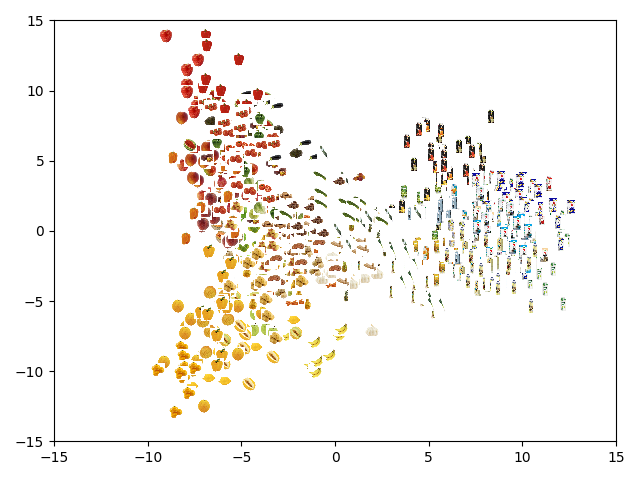
\includegraphics[width=\textwidth]{PaperB/figures_and_tables/latent_space_visualizations/splitae_vcca_comparison/pca_latents_splitae_xiwy_seed2.png}
         \caption{SplitAE$_{xiwy}$}
         \label{fig:splitae_xiwy_comparison}
     \end{subfigure}
     %\hfill
     \begin{subfigure}[b]{0.45\textwidth}
         \centering
         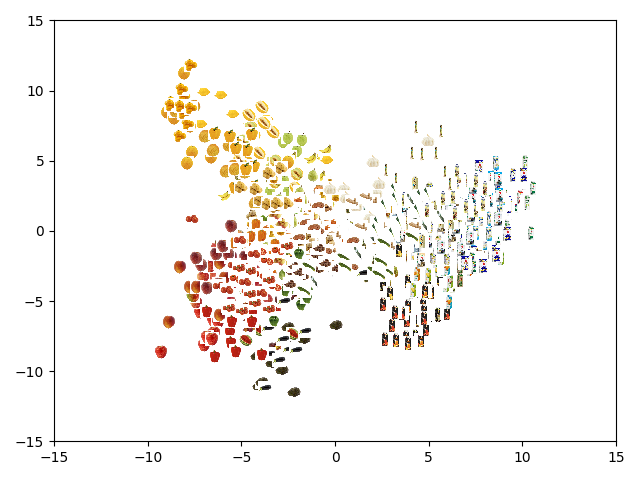
\includegraphics[width=\textwidth]{PaperB/figures_and_tables/latent_space_visualizations/splitae_vcca_comparison/pca_latents_vcca_xiwy_seed2.png}
         \caption{VCCA$_{xiwy}$}
         \label{fig:vcca_xiwy_comparison}
     \end{subfigure} \\
     %\hfill
     \begin{subfigure}[b]{0.45\textwidth}
         \centering
         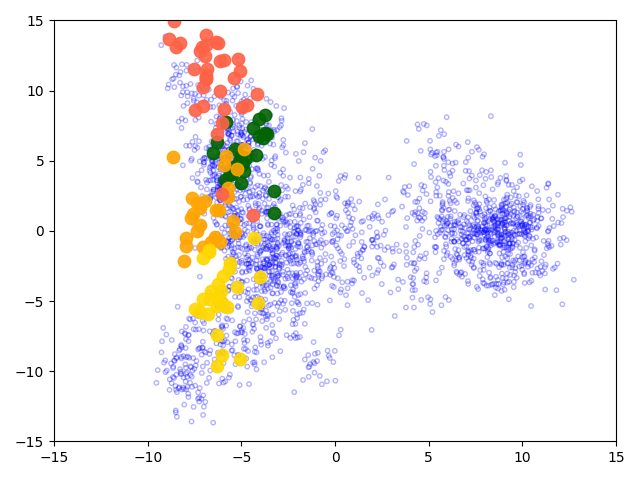
\includegraphics[width=\textwidth]{PaperB/figures_and_tables/latent_space_visualizations/splitae_vcca_comparison/pca_latent_peppers_splitae_xiwy_seed2.png}
         \caption{SplitAE$_{xiwy}$}
         \label{fig:splitae_xiwy_bell_peppers_comparison}
     \end{subfigure}
     \begin{subfigure}[b]{0.45\textwidth}
         \centering
         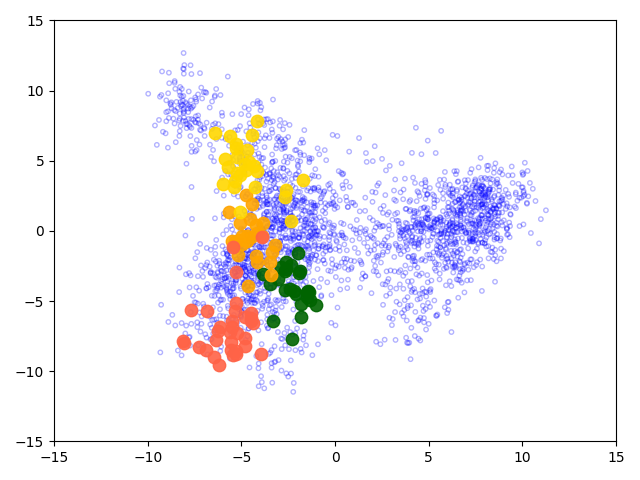
\includegraphics[width=\textwidth]{PaperB/figures_and_tables/latent_space_visualizations/splitae_vcca_comparison/pca_latent_peppers_vcca_xiwy_seed2.png}
         \caption{VCCA$_{xiwy}$}
         \label{fig:vcca_xiwy_bell_peppers_comparison}
     \end{subfigure}
        \caption{Visualizations of the latent representations of the test set from SplitAE$_{xiwy}$ and VCCA$_{xiwy}$. We plot the corresponding iconic image to each latent representation in Figure \ref{fig:splitae_xiwy_comparison} and \ref{fig:vcca_xiwy_comparison}. In Figure \ref{fig:splitae_xiwy_bell_peppers_comparison} and \ref{fig:vcca_xiwy_bell_peppers_comparison}, we plot the bell pepper representations according to the color of the class, while the blue points correspond to the other grocery items. Abbreviations: SplitAE, Split Autoencoder; VCCA, Variational Canonical Correlation Analysis.}
        \label{fig:2d_visualizations_pca_splitae_vcca_comparison}
\end{figure}

We observe that VCCA models compete with their corresponding SplitAE models in the classification task. The main difference between these models is the Kullback-Leibler (KL) divergence~\citeB{B:kullback1951information} term in the ELBO that encourages a smooth latent space for VCCA (see Section \ref{paperB:sec:experimental_procedures}). %Experimental Procedures). 
In contrast, SplitAE learns a latent space that best reconstructs the input data, which can result in parts of the space that does not represent the observed data. We showcase these differences by plotting the latent representations of SplitAE$_{x i w y}$ and VCCA$_{x i w y}$ using PCA in Figure \ref{fig:2d_visualizations_pca_splitae_vcca_comparison}. In Figure \ref{fig:splitae_xiwy_comparison} and \ref{fig:vcca_xiwy_comparison}, we have plotted the corresponding iconic image for the latent representations. We observe that VCCA$_{x i w y}$ tries to establish a smooth latent space by pushing visually similar items closer to each other, but at the same time prevent spreading out the representations too far from the origin. Figure \ref{fig:splitae_xiwy_bell_peppers_comparison} and \ref{fig:vcca_xiwy_bell_peppers_comparison} shows the positions of the bell peppers items in the latent spaces, where the color of the point corresponds to the specific bell pepper class. In Figure \ref{fig:splitae_xiwy_bell_peppers_comparison}, we observe that SplitAE$_{x i w y}$ has spread out the bell peppers across the space, while VCCA$_{x i w y}$ establishes shorter distances between them in Figure \ref{fig:vcca_xiwy_bell_peppers_comparison} due to the regularization.


%%% Figure 5

\begin{figure}[t]
    \centering
    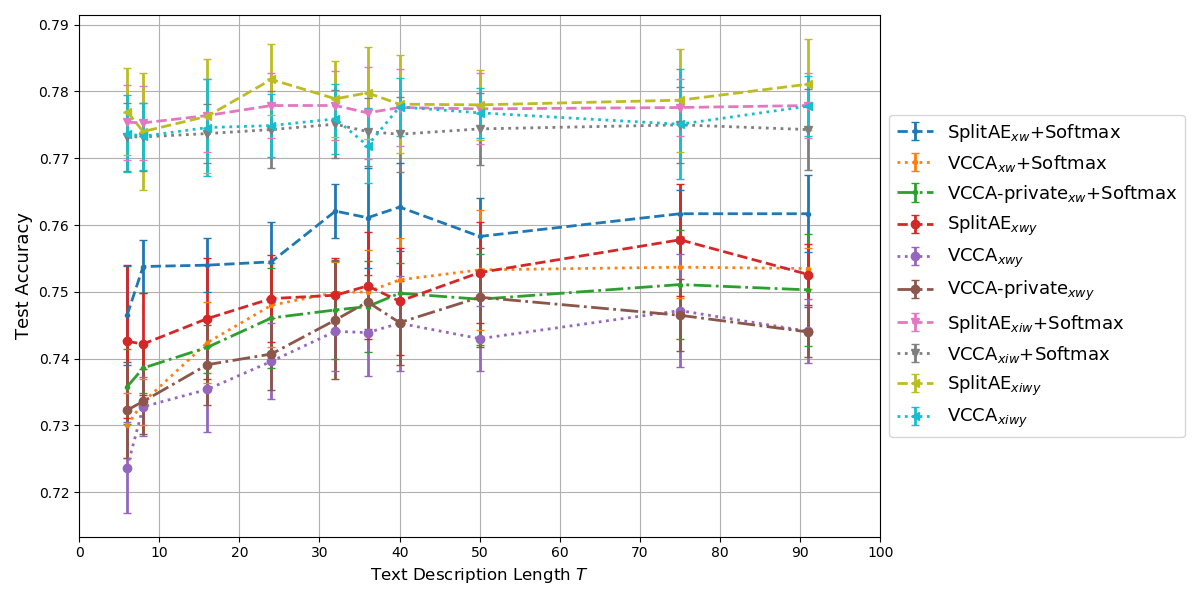
\includegraphics[width=0.95\textwidth]{PaperB/figures_and_tables/varying_t_NEW2.png}
    \caption{Test accuracy over the text description length $T$ for all SplitAE, VCCA, and VCCA-private models using the text description. We show the accuracy for the models trained with $T = 6, 8, 16, 24, 32, 36, 40, 50, 75$, and $91$ words. The results have been averaged for 10 different seeds and the error bars show the standard deviations for every setting of $T$. Abbreviations: SplitAE, Split Autoencoder; VCCA, Variational Canonical Correlation Analysis.}
    \label{fig:varying_t}
\end{figure}


We evaluated the classification performance achieved by each SplitAE, VCCA, and VCCA-private model using the text descriptions with different description lengths $T$. Figure \ref{fig:varying_t} shows the fine-grained classification accuracies for the concerned models. For models using only the text descriptions, the classification accuracies increase as $T$ increases in most cases. Setting $T \geq 32$ results in good classification performance, potentially since the models have learned to separate the grocery items based on that the text descriptions have become more dissimilar and unique. The classification accuracies are mostly stable as $T$ varies for the models with the additional iconic images. Since including iconic images significantly increases the classification performance over models only using text descriptions, we conclude that the iconic images are more helpful when we want to classify the grocery items from natural images. 





\begin{figure}[t]
     \centering
     \begin{subfigure}[b]{0.3\textwidth}
         \centering
         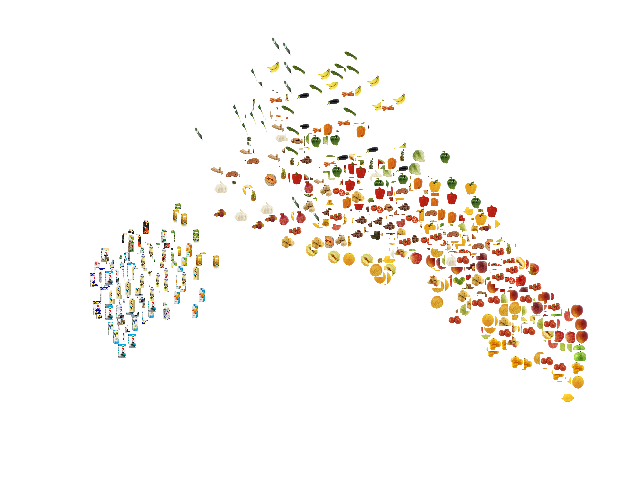
\includegraphics[width=\textwidth]{PaperB/figures_and_tables/latent_space_visualizations/pca_densenet.png}
         \caption{DenseNet169}
         \label{fig:pca_densenet}
     \end{subfigure}
     \begin{subfigure}[b]{0.3\textwidth}
         \centering
         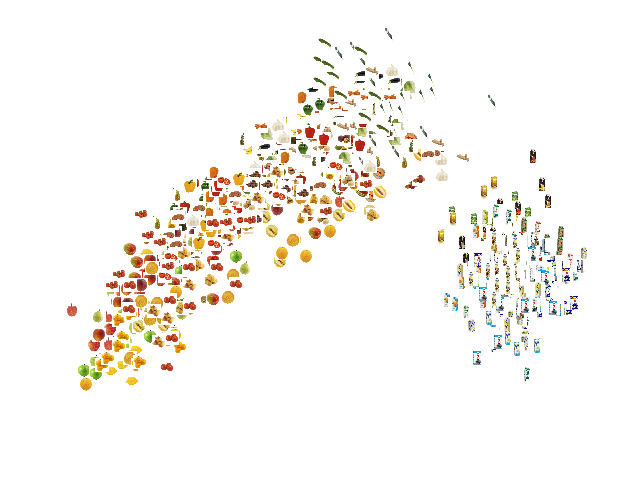
\includegraphics[width=\textwidth]{PaperB/figures_and_tables/latent_space_visualizations/pca_latents_vae_seed2.png}
         \caption{VAE$_{x}$}
         \label{fig:pca_vae_x}
     \end{subfigure} 
     \begin{subfigure}[b]{0.3\textwidth}
         \centering
         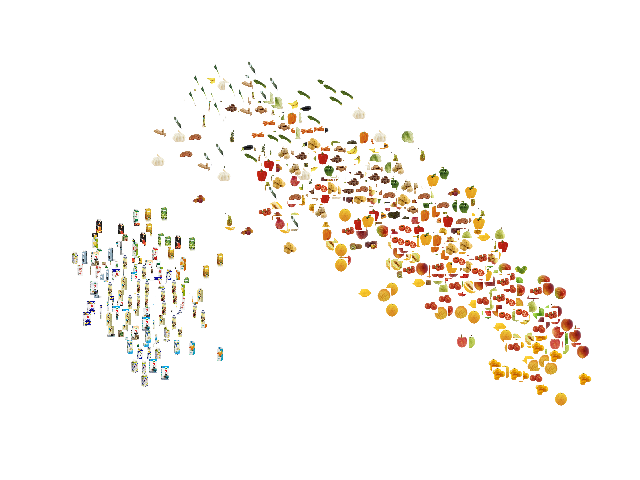
\includegraphics[width=\textwidth]{PaperB/figures_and_tables/latent_space_visualizations/pca_latents_vcca_xy_seed2.png}
         \caption{VCCA$_{x y}$}
         \label{fig:pca_vcca_xy}
     \end{subfigure} \\
     \begin{subfigure}[b]{0.3\textwidth}
         \centering
         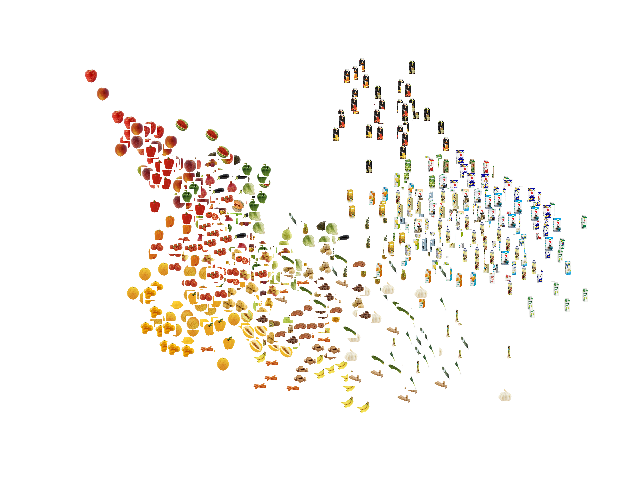
\includegraphics[width=\textwidth]{PaperB/figures_and_tables/latent_space_visualizations/pca_latents_vcca_xi_seed2.png}
         \caption{VCCA$_{x i}$}
         \label{fig:pca_vcca_xi}
     \end{subfigure} 
     \begin{subfigure}[b]{0.3\textwidth}
         \centering
         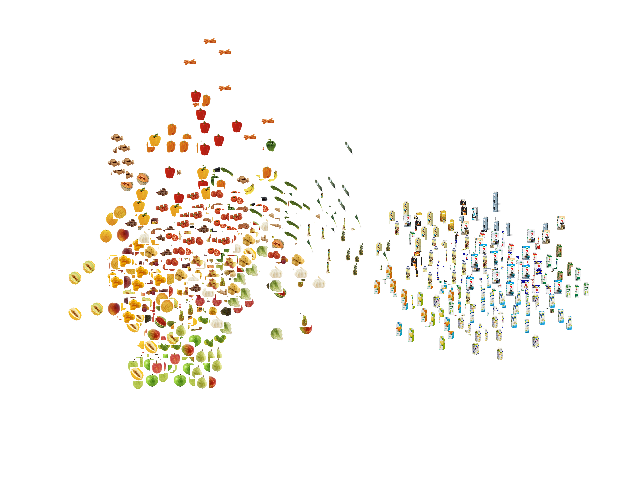
\includegraphics[width=\textwidth]{PaperB/figures_and_tables/latent_space_visualizations/pca_latents_vcca_xw_seed2.png}
         \caption{VCCA$_{x w}$}
         \label{fig:pca_vcca_xw}
     \end{subfigure} 
     \begin{subfigure}[b]{0.3\textwidth}
         \centering
         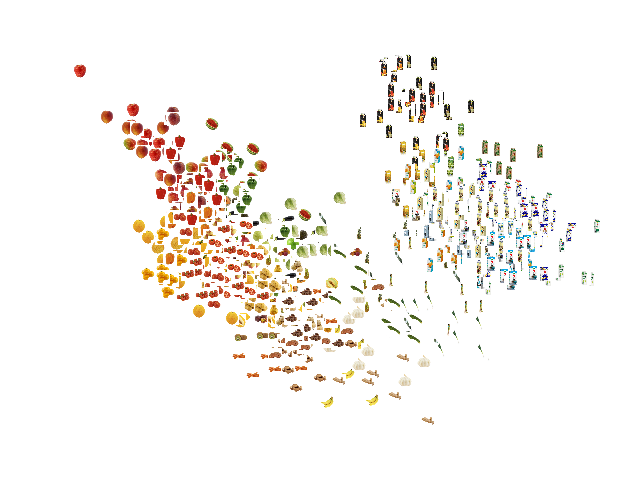
\includegraphics[width=\textwidth]{PaperB/figures_and_tables/latent_space_visualizations/pca_latents_vcca_xiw_seed2.png}
         \caption{VCCA$_{x i w}$}
         \label{fig:pca_vcca_xiw}
     \end{subfigure} \\
     \begin{subfigure}[b]{0.3\textwidth}
         \centering
         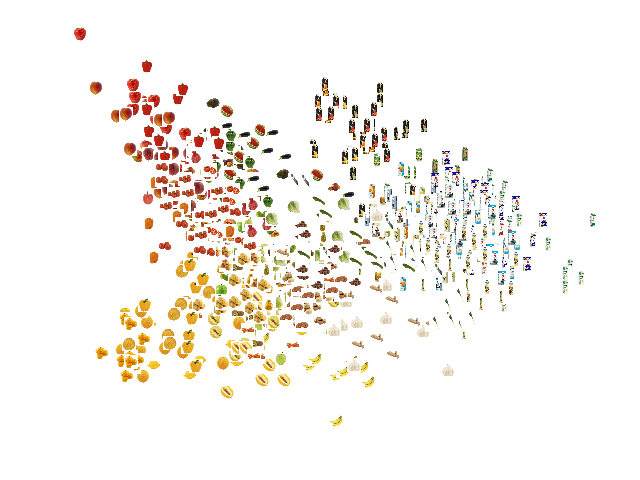
\includegraphics[width=\textwidth]{PaperB/figures_and_tables/latent_space_visualizations/pca_latents_vcca_xiy_seed2.png}
         \caption{VCCA$_{x i y}$}
         \label{fig:pca_vcca_xiy}
     \end{subfigure} 
     \begin{subfigure}[b]{0.3\textwidth}
         \centering
         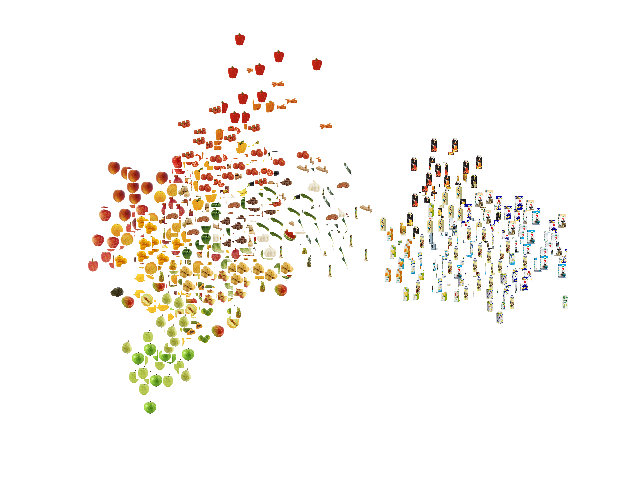
\includegraphics[width=\textwidth]{PaperB/figures_and_tables/latent_space_visualizations/pca_latents_vcca_xwy_seed2.png}
         \caption{VCCA$_{x w y}$}
         \label{fig:pca_vcca_xwy}
     \end{subfigure} 
     \begin{subfigure}[b]{0.3\textwidth}
         \centering
         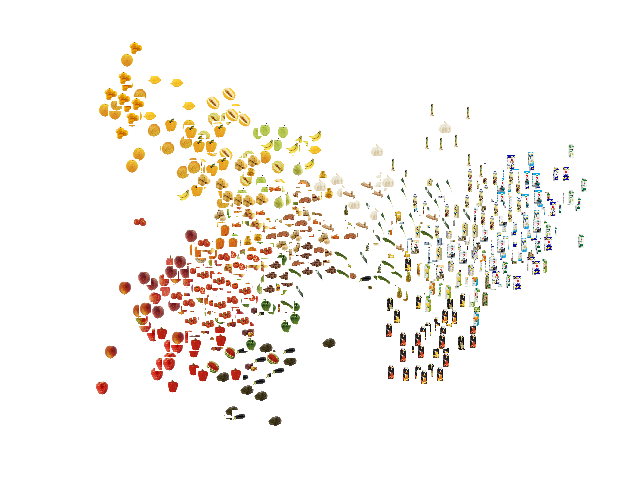
\includegraphics[width=\textwidth]{PaperB/figures_and_tables/latent_space_visualizations/pca_latents_vcca_xiwy_seed2.png}
         \caption{VCCA$_{x i w y}$}
         \label{fig:pca_vcca_xiwy}
     \end{subfigure} 
    \vspace{-2mm}
    \caption{Visualizations of the latent representations from the test set, where we plot the iconic image of the corresponding object classes. We also plot the PCA projection of the natural image features from the off-the-shelf DenseNet169 in Figure \ref{fig:pca_densenet}. All models have been initialized with the same random seed before training. %Abbreviations: VAE, Variational Autoencoder; VCCA, Variational Canonical Correlation Analysis.
    }
    \label{fig:2d_visualizations_pca}
    \vspace{-3mm}
\end{figure}


\subsection{Investigation of the Learned Representations}
\label{paperB:sec:investigation_of_the_learned_representations}

To gain insights about the effects that each view has on the classification performance, we visualize the latent space by plotting the latent representations using PCA. Utilizing the additional views showed to have similar effects on the structure of the latent spaces from SplitAE and VCCA. 
Since our main interest lies in representation learning with variational methods, we focus on studying the latent representations of VCCA and VCCA-private. 
Firstly, we use PCA to visualize the latent representations in 2D and plot the corresponding iconic images of the representations (see Figure \ref{fig:2d_visualizations_pca}). Secondly, to illustrate the effects that the iconic images and text descriptions have on the learned latent space, we focus on two cases of grocery items where one of the views helps to separate two different types of classes and the other one does not (see Figure \ref{fig:2d_visualizations_pca_apples} and \ref{fig:2d_visualizations_pca_juice_yoghurt}). Finally, we look into the shared and private latent spaces learned by VCCA-private$_{x w}$ and observe that variations in image backgrounds and structures of text sentences have been separated from the shared representations into the private ones. 

In Figure \ref{fig:2d_visualizations_pca}, we show the latent representations for the VCCA models that were used in Table \ref{tab:classification_results_on_test_set} (see subsection Classification Results in Results).
%(see Section \ref{sec:classification_results}). 
We also plot the PCA projections of the natural image features from the off-the-shelf DenseNet169 in Figure \ref{fig:pca_densenet} as a baseline. Figure \ref{fig:pca_vae_x} and \ref{fig:pca_vcca_xy} shows the latent space learned by n VAE$_{x}$ and VCCA$_{x y}$, which are similar to the DenseNet169 feature space since these models are performing compression of the natural image features into the learned latent space. We observe that these models have divided packages and raw food items into two separate clusters. However, the fruits and vegetables are scattered across their cluster and the packages have been grouped close to each other despite having different colors, e.g., black and white, on the cartons. 

The structure of the latent spaces becomes distinctly different for the VCCA models that use either iconic images or text descriptions as an additional view and we can observe the different structures that the views bring to the learned latent space. In Figure \ref{fig:pca_vcca_xi} and \ref{fig:pca_vcca_xiy}, we see that visually similar objects, in terms of color and shape, have moved closer together by utilizing iconic images in VCCA$_{x i}$ and VCCA$_{x i y}$. When using text descriptions in VCCA$_{x w}$ and VCCA$_{x w y}$, we also observe in the fruit and vegetable cluster that the items are more grouped based on their color in Figure \ref{fig:pca_vcca_xw} and \ref{fig:pca_vcca_xwy}. 
Figure \ref{fig:pca_vcca_xiw} and \ref{fig:pca_vcca_xiwy} shows the latent spaces in VCCA$_{x i w}$ and VCCA$_{x i w y}$ respectively. These latent spaces are similar to the ones learned by VCCA$_{x i}$ and VCCA$_{x i y}$ in the sense that these latent spaces also group items based on their color and shape. We believe that this structure imposed by the iconic images could be softened by reducing the scaling weight $\lambda_{i}$, which potentially could reduce the classification accuracy as a consequence. The difference between the latent spaces is not evident comparing the models using the class label.

\vspace{-3mm}
\paragraph{Red and Green Apples} To showcase how the iconic images help to learn good representations, we consider all of the apple classes in the dataset, namely the red apples \textit{Pink Lady}, \textit{Red Delicious} and \textit{Royal Gala}, and also the green apples \textit{Golden Delicious} and \textit{Granny Smith}. In Figure \ref{fig:2d_visualizations_pca_apples}, we group the red apple classes and visualize their latent representations by red points. The green apples are grouped similarly and we visualize their latent representations with green points. Latent representations of all other grocery items are visualized as blue points. The models using iconic images as one view in Figure \ref{fig:pca_vcca_xi_apples}, \ref{fig:pca_vcca_xiy_apples}, \ref{fig:pca_vcca_xiw_apples}, and \ref{fig:pca_vcca_xiwy_apples} have managed to separate the red and green apples based on their color differences. The models using text description have instead moved the apples closer together in one part of the latent space, possibly because of their similarities mentioned in the description. 

%%% Figure 7



\begin{figure}[t]
     \centering
     \begin{subfigure}[b]{0.3\textwidth}
         \centering
         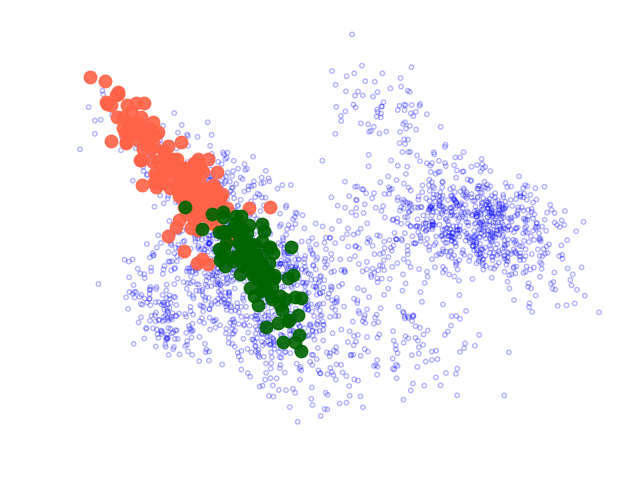
\includegraphics[width=\textwidth]{PaperB/figures_and_tables/latent_space_visualizations/apples_new/pca_latent_apples_vcca_xi_seed2.png}
         \caption{VCCA$_{x i}$}
         \label{fig:pca_vcca_xi_apples}
     \end{subfigure} 
     \begin{subfigure}[b]{0.3\textwidth}
         \centering
         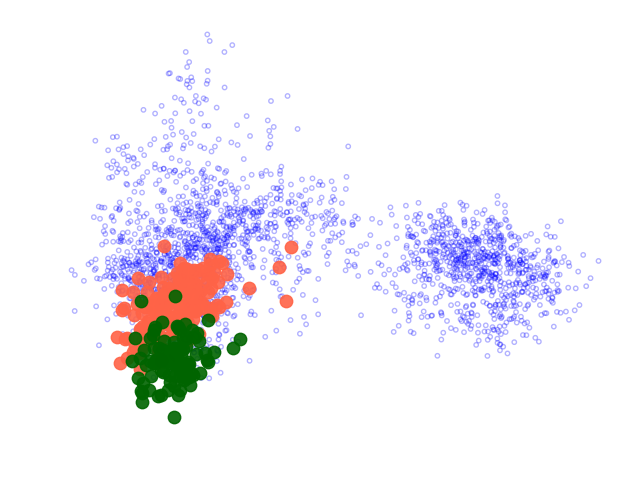
\includegraphics[width=\textwidth]{PaperB/figures_and_tables/latent_space_visualizations/apples_new/pca_latent_apples_vcca_xw_seed2.png}
         \caption{VCCA$_{x w}$}
         \label{fig:pca_vcca_xw_apples}
     \end{subfigure} 
     \begin{subfigure}[b]{0.3\textwidth}
         \centering
         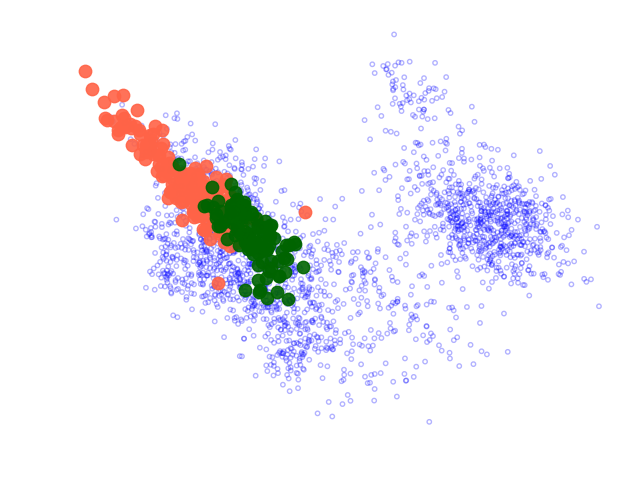
\includegraphics[width=\textwidth]{PaperB/figures_and_tables/latent_space_visualizations/apples_new/pca_latent_apples_vcca_xiw_seed2.png}
         \caption{VCCA$_{x i w}$}
         \label{fig:pca_vcca_xiw_apples}
     \end{subfigure} \\
     \begin{subfigure}[b]{0.3\textwidth}
         \centering
         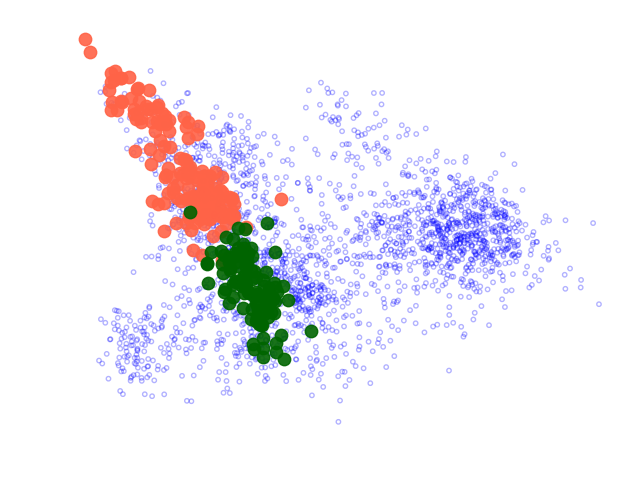
\includegraphics[width=\textwidth]{PaperB/figures_and_tables/latent_space_visualizations/apples_new/pca_latent_apples_vcca_xiy_seed2.png}
         \caption{VCCA$_{x i y}$}
         \label{fig:pca_vcca_xiy_apples}
     \end{subfigure} 
     \begin{subfigure}[b]{0.3\textwidth}
         \centering
         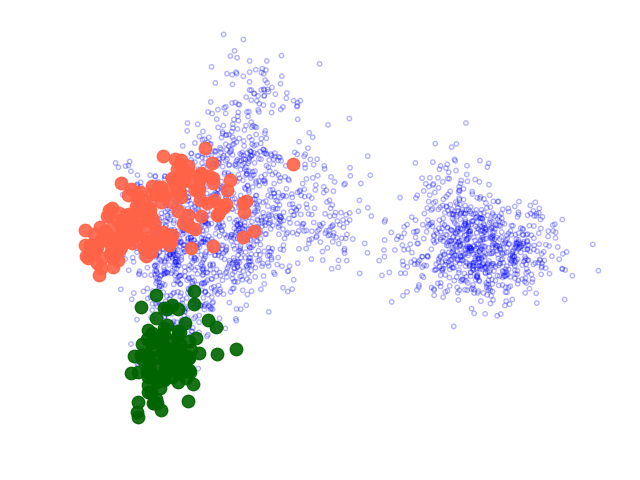
\includegraphics[width=\textwidth]{PaperB/figures_and_tables/latent_space_visualizations/apples_new/pca_latent_apples_vcca_xwy_seed2.png}
         \caption{VCCA$_{x w y}$}
         \label{fig:pca_vcca_xwy_apples}
     \end{subfigure} 
     \begin{subfigure}[b]{0.3\textwidth}
         \centering
         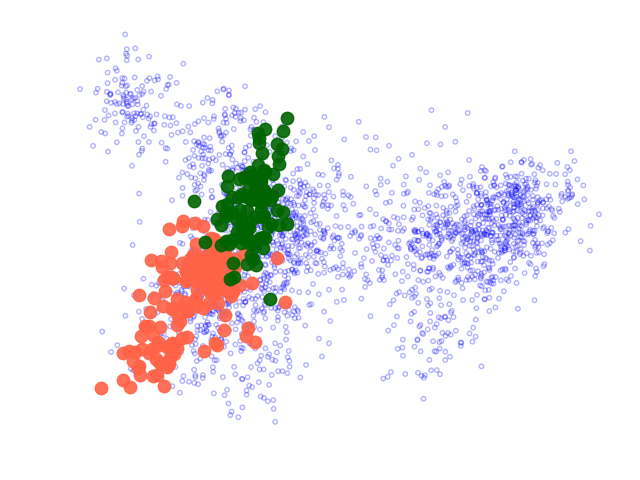
\includegraphics[width=\textwidth]{PaperB/figures_and_tables/latent_space_visualizations/apples_new/pca_latent_apples_vcca_xiwy_seed2.png}
         \caption{VCCA$_{x i w y}$}
         \label{fig:pca_vcca_xiwy_apples}
     \end{subfigure}
    \vspace{-2mm} 
    \caption{Visualizations of the latent representations $\mu_{z}$ of the red and green apples in the Grocery Store dataset. The red points correspond to the red apple classes, while the green points correspond to the green apple. The blue points correspond to the other grocery items. 
    %Abbreviations: VCCA, Variational Canonical Correlation Analysis.
    }
    \label{fig:2d_visualizations_pca_apples}
    \vspace{-3mm}
\end{figure}


\vspace{-3mm}
\paragraph{Juice and Yoghurt Packages} To illustrate how the text descriptions can establish more useful latent representations, we consider a selection of juice and yoghurt classes. These packaged items have similar shapes and colors, which makes it difficult for a classifier to distinguish their content differences using only visual input. In Figure \ref{fig:2d_visualizations_pca_juice_yoghurt}, we visualize the latent representations of the juice and yoghurt packages using yellow and green points respectively. We observe that only VCCA$_{x w}$ and VCCA$_{x w y}$ manages to separate the packages in Figure \ref{fig:pca_vcca_xw_juice_yoghurt} and \ref{fig:pca_vcca_xwy_juice_yoghurt} due to their different text descriptions. Since the iconic images of the packages are visually similar, adding this information is insufficient for separating these packages in the latent space. This indicates that we gain different benefits from the iconic images and text descriptions when it comes to classifying grocery items.

%%% Figure 8


\begin{figure}[t]
     \centering
     \begin{subfigure}[b]{0.3\textwidth}
         \centering
         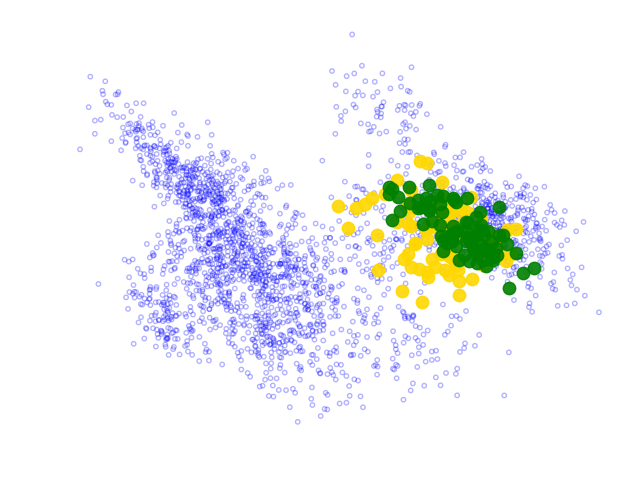
\includegraphics[width=\textwidth]{figures_and_tables/latent_space_visualizations/juice_yoghurt_new/pca_latent_juice_yoghurt_vcca_xi_seed2.png}
         \caption{VCCA$_{x i}$}
         \label{fig:pca_vcca_xi_juice_yoghurt}
     \end{subfigure} 
     \begin{subfigure}[b]{0.3\textwidth}
         \centering
         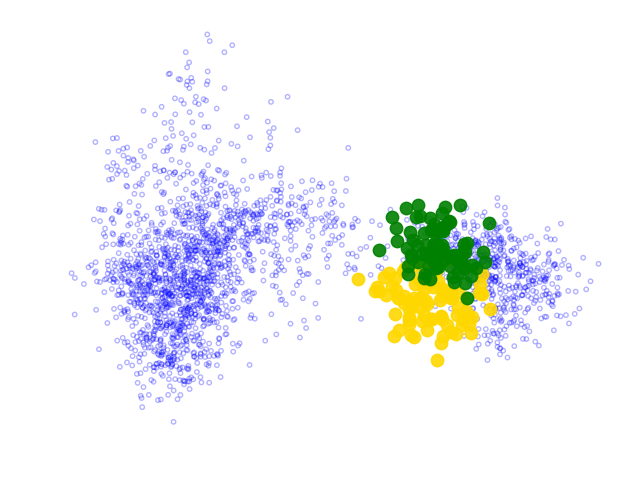
\includegraphics[width=\textwidth]{figures_and_tables/latent_space_visualizations/juice_yoghurt_new/pca_latent_juice_yoghurt_vcca_xw_seed2.png}
         \caption{VCCA$_{x w}$}
         \label{fig:pca_vcca_xw_juice_yoghurt}
     \end{subfigure} 
     \begin{subfigure}[b]{0.3\textwidth}
         \centering
         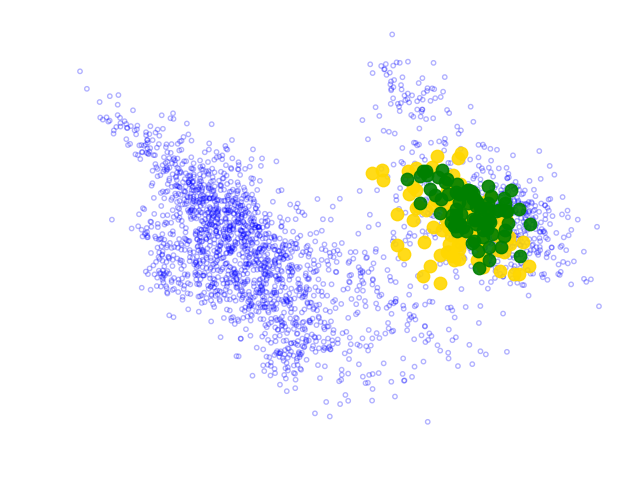
\includegraphics[width=\textwidth]{figures_and_tables/latent_space_visualizations/juice_yoghurt_new/pca_latent_juice_yoghurt_vcca_xiw_seed2.png}
         \caption{VCCA$_{x i w}$}
         \label{fig:pca_vcca_xiw_juice_yoghurt}
     \end{subfigure} \\
     \begin{subfigure}[b]{0.3\textwidth}
         \centering
         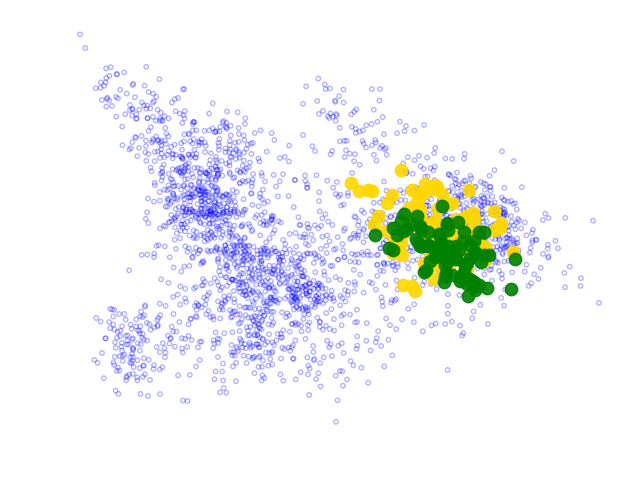
\includegraphics[width=\textwidth]{figures_and_tables/latent_space_visualizations/juice_yoghurt_new/pca_latent_juice_yoghurt_vcca_xiy_seed2.png}
         \caption{VCCA$_{x i y}$}
         \label{fig:pca_vcca_xiy_juice_yoghurt}
     \end{subfigure} 
     \begin{subfigure}[b]{0.3\textwidth}
         \centering
         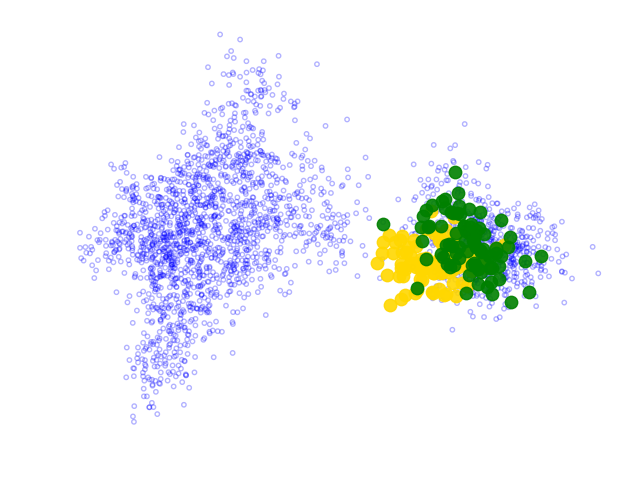
\includegraphics[width=\textwidth]{figures_and_tables/latent_space_visualizations/juice_yoghurt_new/pca_latent_juice_yoghurt_vcca_xwy_seed2.png}
         \caption{VCCA$_{x w y}$}
         \label{fig:pca_vcca_xwy_juice_yoghurt}
     \end{subfigure} 
     \begin{subfigure}[b]{0.3\textwidth}
         \centering
         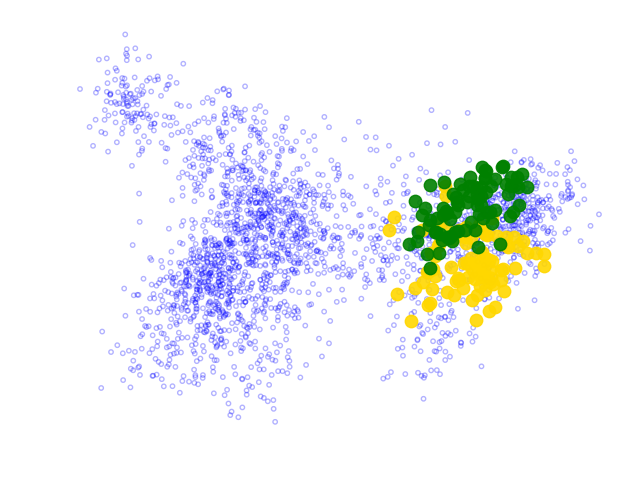
\includegraphics[width=\textwidth]{figures_and_tables/latent_space_visualizations/juice_yoghurt_new/pca_latent_juice_yoghurt_vcca_xiwy_seed2.png}
         \caption{VCCA$_{x i w y}$}
         \label{fig:pca_vcca_xiwy_juice_yoghurt}
     \end{subfigure} 
    \caption{Visualizations of the latent representations $\mu_{z}$ of a selection of juice packages and yoghurt packages in the Grocery Store dataset. The yellow and green points correspond to the juice and yoghurt packages respectively. The blue points correspond to the other grocery items. Abbreviations: VCCA, Variational Canonical Correlation Analysis.}
    \label{fig:2d_visualizations_pca_juice_yoghurt}
\end{figure}



\vspace{-3mm}
\paragraph{Latent Spaces of VCCA-private } We show the shared and private latent spaces of VCCA-private$_{x w}$ in Figure \ref{fig:2d_visualizations_pca_vcca_private_xw}b-d, as well as the single latent space of VCCA$_{x w}$ for comparison in Figure \ref{fig:pca_vcca_xw_z}. 
Comparing with the latent space of VCCA$_{x w}$, the shared latent space of VCCA-private$_{x w}$ in Figure \ref{fig:pca_vcca_private_xw_z}, has structured the raw food items based on their class, color, and shape better than standard VCCA$_{x w}$. In Figure \ref{fig:pca_vcca_private_xw_ux}, we plot the natural images corresponding to the latent representation for the private latent variable $u_{x}$. We zoom in on some natural images and found that the images are structured based on their similarities in background and camera view. On the left and bottom sides of the cluster, we found images of grocery items closely packed together in bins. Single items that are held in the hand of the photographer are placed on the right side, whereas images of items and the store floor are placed on the top and middle of the latent space. The model has therefore managed to separate the variations within the natural image view into the private latent variable $u_{x}$ from the shared latent variable $z$, which probably is the main reason why similar raw food items are closer to each other in Figure \ref{fig:pca_vcca_private_xw_z} than in Figure \ref{fig:pca_vcca_xw_z}. We also plot the corresponding iconic image on the position of the text description representation for the private latent variable $u_{w}$ in Figure \ref{fig:pca_vcca_private_xw_uw}. Note that every text description is projected at the same location in the latent space since the text descriptions are the same for every class item. We highlighted some specific words in the descriptions and observed that descriptions with the same words are usually close to each other. Visually dissimilar items can be grouped close to each other in this latent space, which indicates that the private latent variable $u_{w}$ contains information about the structure of the text sentences, i.e., word occurrences and how they are ordered in the text description. 
In Figure \ref{paperB:fig:2d_visualizations_pca_vcca_private_xi}, %S4, 
we show the shared and private latent spaces of VCCA-private$_{x i}$ and provide a conclusion to the results in Section \ref{paperB:app:investigating_latent_representations_in_vcca_private_xi}. %the Supplemental Experimental Procedures.
%supplementary material.
%In Appendix \ref{app:investigating_latent_representations_in_vcca_private_xi}, we show the shared and private latent spaces of VCCA-private$_{x i}$ in \MK{Figure S14} and provide a conclusion to the results.

%%%% Figure 9

\begin{figure}[!tp]
     \centering
     \begin{subfigure}[b]{0.49\textwidth}
         \centering
         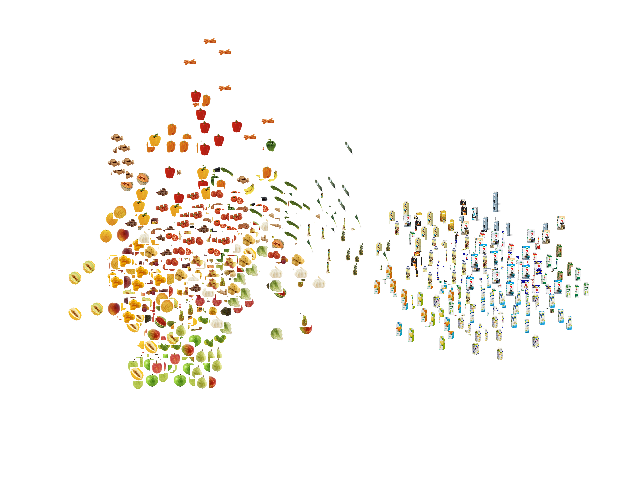
\includegraphics[width=\textwidth]{PaperB/figures_and_tables/latent_space_visualizations/pca_latents_vcca_xw_seed2.png}
         \caption{$\mu_{z}$ from VCCA$_{x w}$}
         \label{fig:pca_vcca_xw_z}
     \end{subfigure} 
     \begin{subfigure}[b]{0.49\textwidth}
         \centering
         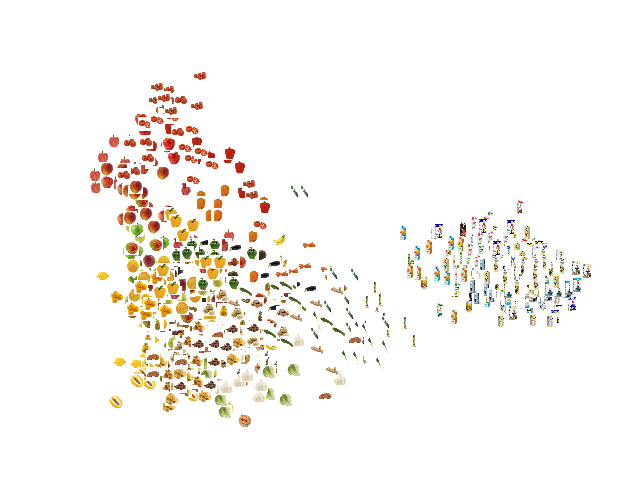
\includegraphics[width=\textwidth]{PaperB/figures_and_tables/private_latent_space_visualizations/pca_z_vaecca_private_xw_seed1.png}
         \caption{$\mu_{z}$ from VCCA-private$_{x w}$}
         \label{fig:pca_vcca_private_xw_z}
     \end{subfigure} \\
     \begin{subfigure}[b]{0.6\textwidth}
         \centering
         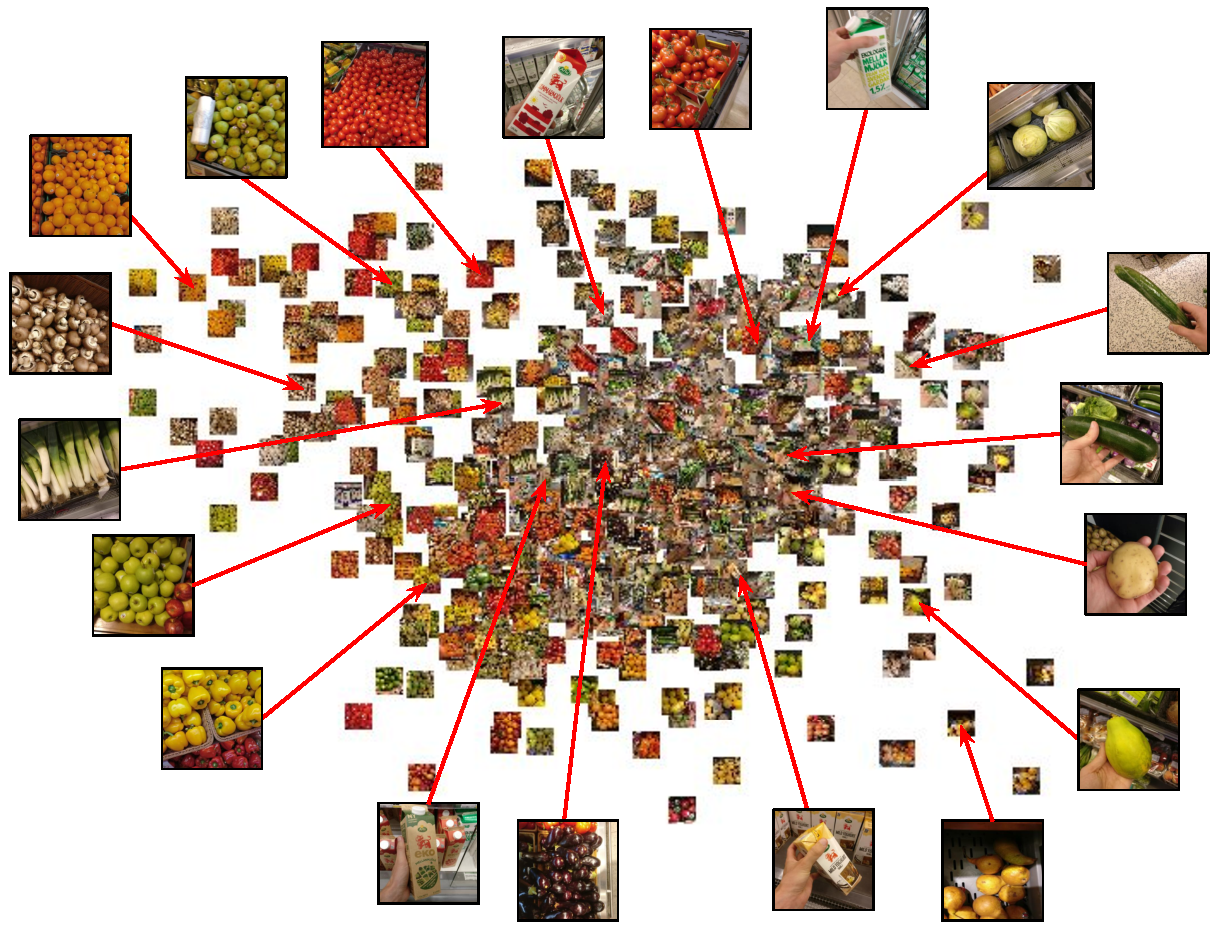
\includegraphics[width=\textwidth]{PaperB/figures_and_tables/private_latent_space_visualizations/vcca_private_ux_space.pdf}
         \caption{$\mu_{x}$ from VCCA-private$_{x w}$}
         \label{fig:pca_vcca_private_xw_ux}
     \end{subfigure} \\
     \begin{subfigure}[b]{0.7\textwidth}
         \centering
         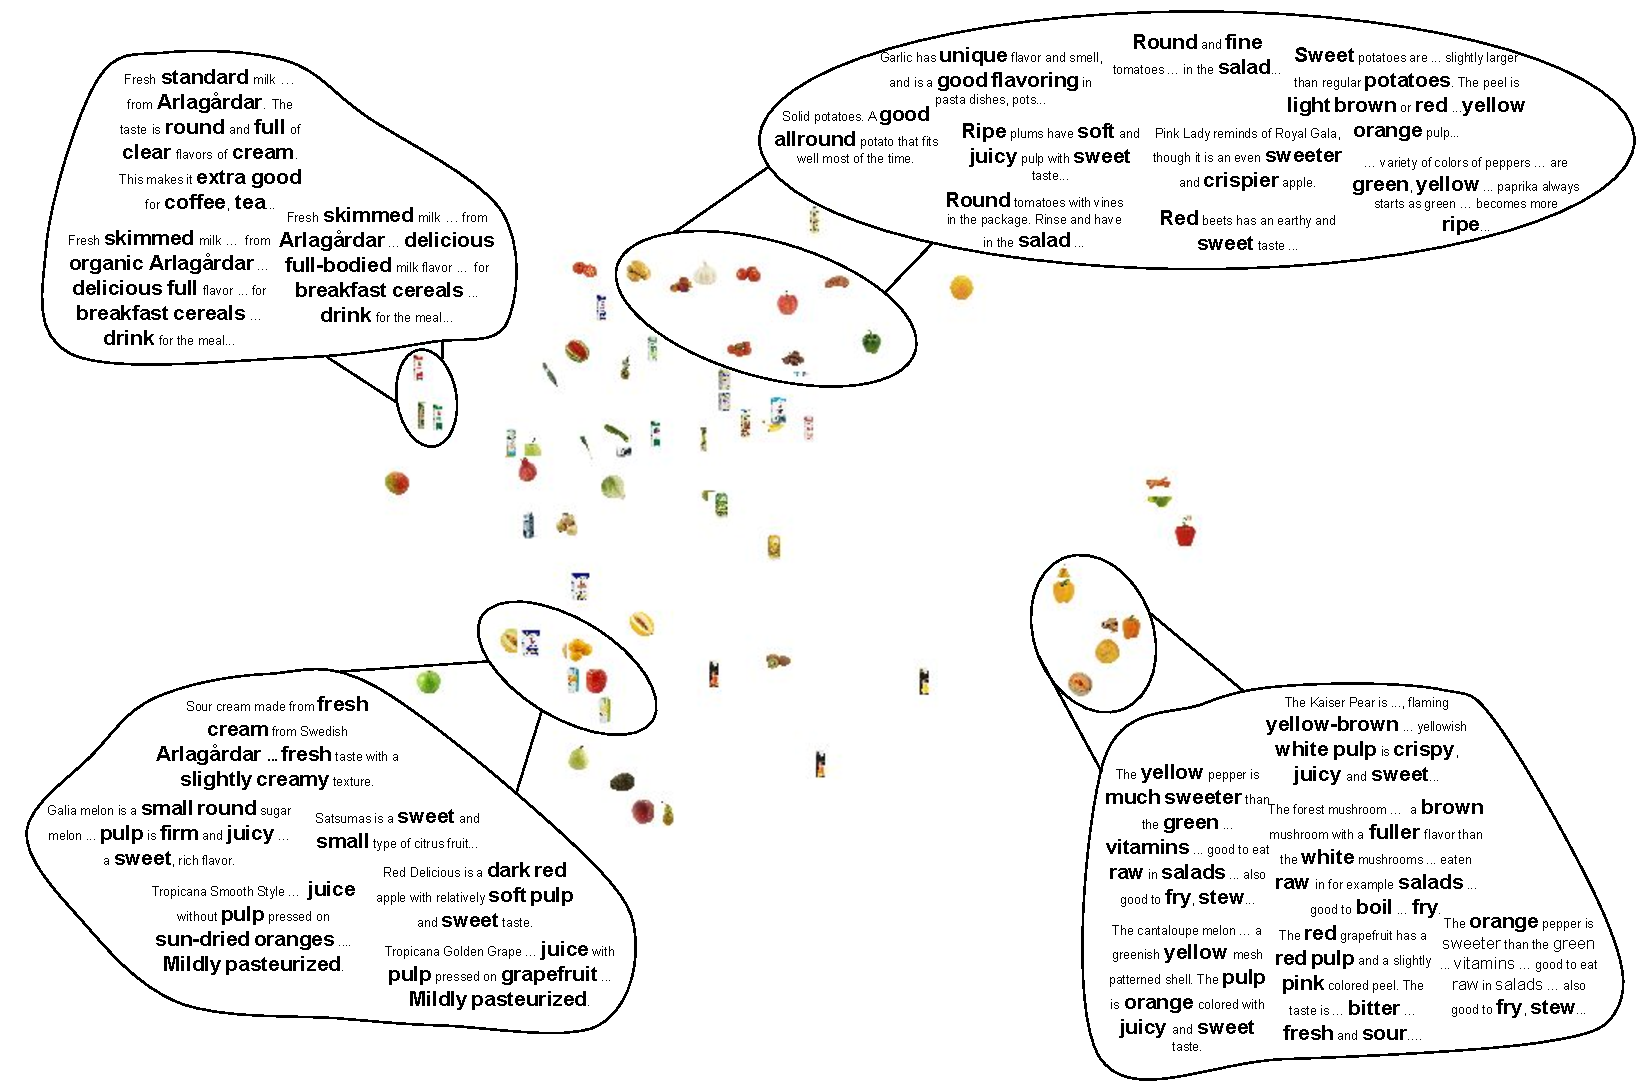
\includegraphics[width=\textwidth]{PaperB/figures_and_tables/private_latent_space_visualizations/vcca_private_uw_space.pdf}
         \caption{$\mu_{w}$ from VCCA-private$_{x w}$}
         \label{fig:pca_vcca_private_xw_uw}
     \end{subfigure} 
    \caption{Visualizations of the latent representations $\mu_{z}$ of a selection of juice packages and yoghurt packages in the Grocery Store dataset. The yellow and green points correspond to the juice and yoghurt packages respectively. The blue points correspond to the other grocery items. 
    	%Abbreviations: VCCA, Variational Canonical Correlation Analysis.
    }
    \label{fig:2d_visualizations_pca_vcca_private_xw}
\end{figure}


\renewcommand{\arraystretch}{1.05}
\begin{table}[!th]
\centering
\caption{Results on image quality of decoded iconic images for the Variational Canonical Correlation Analysis (VCCA) models using the iconic images. The subscript letters in the model names indicate the data views used in the model. $\uparrow$ denotes higher is better, $\downarrow$ lower is better. Peak Signal-to-Noise Ratio (PSNR), Structural Similarity (SSIM), and Kullback-Leibler (KL) divergence are measured by comparing the true iconic image against the decoded one. Accuracy shows the classification performance for each model and has been taken from Table \ref{tab:classification_results_on_test_set}. We report means and standard deviations averaged over 10 random seeds for all metrics.
}
\vspace{-2mm}
\begin{tabular}{l c c c c }
    \hline
    Model & PSNR $\uparrow$ & SSIM $\uparrow$ & KL $\downarrow$ &  Accuracy (\%) $\uparrow$  \\ \hline
    VCCA$_{x i}$ & $20.13 \pm 0.05$ & $0.72 \pm 0.00$ & $4.43 \pm 0.21$ & $77.02 \pm \, 0.51$  \\ 
    \rowcolor{gray!30}
    VCCA$_{x i y}$ & $20.12 \pm 0.09$ & $0.73 \pm 0.00$ & $4.35 \pm 0.22$ & $77.22 \pm 0.55$  \\ 
    VCCA$_{x i w}$ & $20.11 \pm 0.09$ & $0.73 \pm 0.00$ & $4.29 \pm 0.24$ & $77.51 \pm 0.51$  \\
    \rowcolor{gray!30}
    VCCA$_{x i w y}$ & $20.16 \pm 0.08$ & $0.73 \pm	0.00$ & $4.32 \pm 0.22$ & $77.78 \pm 0.45$  \\  
    \hline
\end{tabular}
\label{tab:iconic_image_similarity_metrics}
\vspace{-3mm}
\end{table}

\subsection{Decoding Iconic Images from Unseen Natural Images}
\label{paperB:sec:decoding_iconic_images} 

In this section, we show how the iconic image decoder can decode plausible iconic images of grocery items from unseen natural images in the test set. We apply the same approach as in~\citeB{B:klasson2019hierarchical}, where we encode unseen natural images and then decode the retrieved latent representation back into an iconic image. We also report several image similarity metrics to investigate if the decoded image quality is correlated with classification performance.
We report peak signal-to-noise ratio (PSNR), structural similarity (SSIM)~\citeB{B:wang2004image}, and the KL divergence by comparing the decoded iconic images to the true ones. For computing the KL divergence, we model the decoded and true iconic image using two Gaussian Mixture Model (GMM)~\citeB{B:cui2015comparison, B:goldberger2003efficient}. The images are then represented as density functions, such that we can measure the similarity between the two densities with the KL divergence and use it as an image similarity metric. Since the KL divergence between two GMMs is not analytically tractable, we apply Monte Carlo simulation using $n$ i.i.d. samples drawn from the decoded image density for approximating the KL divergence~\citeB{B:hershey2007approximating}. 
Due to the simple structure of the iconic images, we fit the GMMs with $K=2$ Gaussian components using the RGB color values and draw $n=100$ Monte Carlo samples to estimate the KL divergence in all experiments. 
Table \ref{tab:iconic_image_similarity_metrics} shows the image similarity metrics between the VCCA models using the iconic images. We also show the model classification accuracy for each model, which have been taken from Table \ref{tab:classification_results_on_test_set}. 
The models perform on par on the image similarity metrics, which indicates that the quality of the decoded images is intact if the model extends to utilizing text descriptions and class labels in addition to the iconic images.

%In Figure \ref{fig:decoded_iconic_images_with_metrics}, 
In Table \ref{tab:decoded_iconic_images_with_metrics}, we display five different natural images from the test set, their true corresponding iconic image, the decoded iconic image from VCCA$_{x i w y}$. 
We also show the true and predicted labels from the class label decoder (see Pred. Label). 
Additionally, we report the image similarity metrics PSNR, SSIM, and KL divergence between the decoded and true iconic images. For the Mango and Royal Gala images, we observe that the decoded images are visually plausible, in terms of recognized item, color, and shape, in both cases, which coheres with the high PSNR and SSIM values and low KL values.
The third row shows a shelf with orange and green bell peppers where the decoded image has indeed been decoded into a mix of a green and orange bell pepper. In the two succeeding rows, we display failure cases where the model confuses the true class label with other grocery items. We observe that each metric drops according to the mismatch between decoded and true iconic images. The fourth row shows a basket of Anjou pears, where the model confuses the pear with a Granny Smith apple which can be seen in the decoded image. In the fifth row, there are red milk packages stacked behind a handheld sourcream package, where the decoded image becomes a blurry mix of the milk and sourcream package. Although the predicted class is incorrect, we observe that the prediction is reasonable based on the decoded iconic image.


\begin{table}[t]
	\centering
	\caption{Examples of decoded iconic images from VCCA$_{\vx \vi \vw \vy}$ with their corresponding natural image and true iconic image as well as predicted labels and image similarity metrics. The column {\bf Classification} shows the true label for the natural image (True Label) and the label predicted by the model (Pred. Label). The column {\bf Metrics} shows PSNR, SSIM, and KL divergence between the decoded and true iconic images. }
	\vspace{-2mm}
	\resizebox{0.98\textwidth}{!}{
		
\begin{tabular}{c c c c c}
	\toprule 
	{\bf Natural Image} & {\bf Iconic Image} &
	{\bf Decoded Image} & {\bf Classification} & {\bf Metrics}  \\
	\midrule 
	\multirow{3}{*}{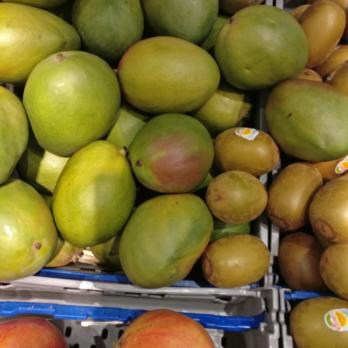
\includegraphics[width=13mm, height=13mm]{PaperB/figures_and_tables/decoded_iconic_images/Mango_002_image477.jpg}} & \multirow{3}{*}{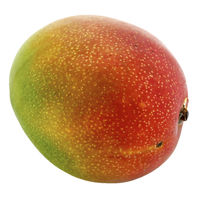
\includegraphics[width=13mm, height=13mm]{PaperB/figures_and_tables/iconic_image_figures/Mango_Iconic.jpg}} & \multirow{3}{*}{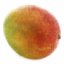
\includegraphics[width=13mm, height=13mm]{PaperB/figures_and_tables/decoded_iconic_images/vcca_xiwy_NEW/mango_image477.png}} & \multirowcell{3}{True Label: Mango\\ \\ Pred. Label: Mango} & PSNR: $25.31$ \\
	& & & & SSIM: $0.88$ \\
	& & & & KL: $0.36$ \\
	
	\midrule
	\multirow{3}{*}{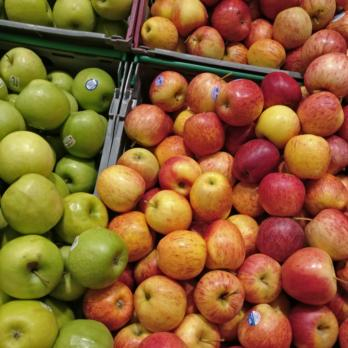
\includegraphics[width=13mm, height=13mm]{PaperB/figures_and_tables/decoded_iconic_images/Royal-Gala_055.jpg}} & \multirow{3}{*}{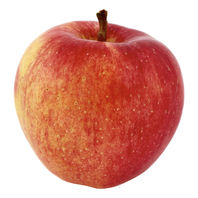
\includegraphics[width=13mm, height=13mm]{PaperB/figures_and_tables/iconic_image_figures/Royal-Gala-Apple_Clean.jpg}} & \multirow{3}{*}{
\includegraphics[width=13mm, height=13mm]{PaperB/figures_and_tables/decoded_iconic_images/vcca_xiwy_NEW/royal_gala_image266.png}} & \multirowcell{3}{True Label: Royal Gala\\ \\ Pred. Label: Royal Gala} & PSNR: $25.72$ \\
	& & & & SSIM: $0.92$ \\
	& & & & KL: $1.73$ \\
	
	\midrule
	\multirow{3}{*}{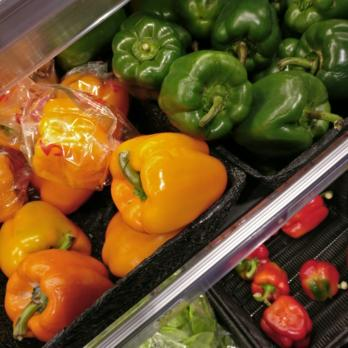
\includegraphics[width=13mm, height=13mm]{PaperB/figures_and_tables/decoded_iconic_images/Orange-Bell-Pepper_008.jpg}} & \multirow{3}{*}{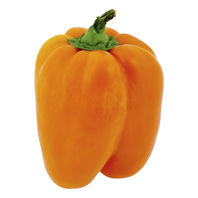
\includegraphics[width=13mm, height=13mm]{PaperB/figures_and_tables/iconic_image_figures/Orange-Bell-Pepper_Iconic.jpg}} & \multirow{3}{*}{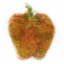
\includegraphics[width=13mm, height=13mm]{PaperB/figures_and_tables/decoded_iconic_images/vcca_xiwy_NEW/orange_bell_pepper_image2191.png}} & \multirowcell{3}{True Label: Orange Bell Pepper\\ \\ Pred. Label: Orange Bell Pepper} & PSNR: $16.64$ \\
	& & & & SSIM: $0.61$ \\
	& & & & KL: $3.74$ \\
	
	\midrule
	\multirow{3}{*}{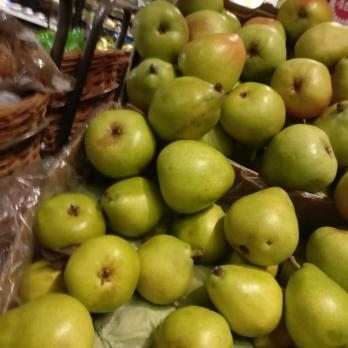
\includegraphics[width=13mm, height=13mm]{PaperB/figures_and_tables/decoded_iconic_images/Anjou_015.jpg}} & \multirow{3}{*}{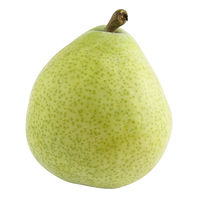
\includegraphics[width=13mm, height=13mm]{PaperB/figures_and_tables/iconic_image_figures/Anjou-Pear_Clean.jpg}} & \multirow{3}{*}{
\includegraphics[width=13mm, height=13mm]{PaperB/figures_and_tables/decoded_iconic_images/vcca_xiwy_NEW/anjou_pear_image849.png}} & \multirowcell{3}{True Label: Anjou\\ \\ Pred. Label: Granny Smith} & PSNR: $14.64$ \\
	& & & & SSIM: $0.51$ \\
	& & & & KL: $28.01$ \\
	
	\midrule
	\multirow{3}{*}{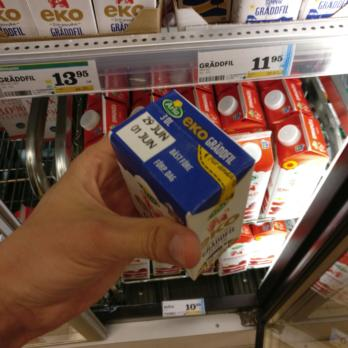
\includegraphics[width=13mm, height=13mm]{PaperB/figures_and_tables/decoded_iconic_images/Arla-Ecological-Sour-Cream_005.jpg}} & \multirow{3}{*}{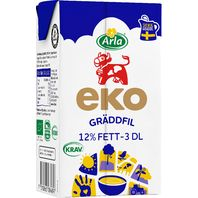
\includegraphics[width=13mm, height=13mm]{PaperB/figures_and_tables/iconic_image_figures/Arla-Ecological-Sour-Cream_Iconic.jpg}} & \multirow{3}{*}{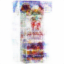
\includegraphics[width=13mm, height=13mm]{PaperB/figures_and_tables/decoded_iconic_images/vcca_xiwy_NEW/arla_eco_sourcream_image1565.png}} & \multirowcell{3}{True Label: Arla Eco. Sourcream\\ \\ Pred. Label: Arla Std. Milk} & PSNR: $13.16$ \\
	& & & & SSIM: $0.45$ \\
	& & & & KL: $1.33$ \\
	\bottomrule 
\end{tabular}

	}
	\label{tab:decoded_iconic_images_with_metrics}
	\vspace{-3mm}
\end{table}

%
\begin{figure}[t]
    \centering
    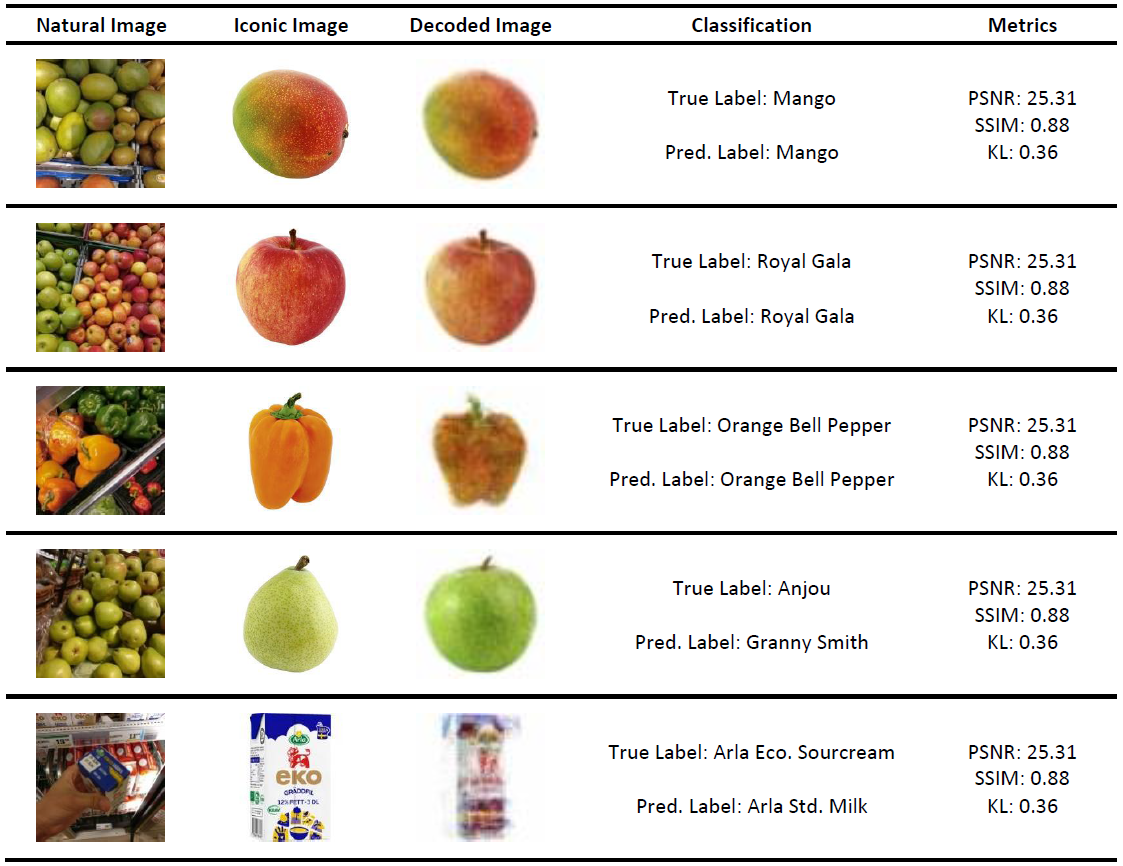
\includegraphics[width=0.95\textwidth]{PaperB/figures_and_tables/figure10.png}
    \vspace{-2mm}
    \caption{Examples of decoded iconic images from VCCA$_{xiwy}$ with their corresponding natural image and true iconic image as well as predicted labels and image similarity metrics. The column Classification shows the true label for the natural image (True Label) and the label predicted by the model (Pred. Label). %Abbreviations: VCCA, Variational Canonical Correlation Analysis; PSNR, Peak Signal-to-Noise Ratio; SSIM, Structural Similarity; KL, Kullback-Leibler Divergence; Arla Eco. Sourcream, Arla Ecological Sourcream; Arla Std. Milk, Arla Standard Milk.
    }
    \label{fig:decoded_iconic_images_with_metrics}
  	\vspace{-3mm}
\end{figure} %% Reported metrics in table were wrong
